% preamble
% report --> small books, reports, etc...
\documentclass{report}

% needed if we want to put images
\usepackage{graphicx}

% used to make the table of contents clickable
\usepackage{hyperref}
\hypersetup{
    colorlinks,
    citecolor=black,
    filecolor=black,
    linkcolor=black,
    urlcolor=black
}

%used to make tables
\usepackage{booktabs}

% let's change this ugly serif font!
\renewcommand{\familydefault}{\sfdefault}



% now start with the RASD document
\begin{document}

\title{\textbf{myTaxiService} \\ -  \\ \textbf{Requirements Analysis and Specification Document}}
\author{Davide Cremona, Simone Deola}
\maketitle

\tableofcontents

\chapter{Introduction}

	\section{Purpose}
	This document is the R.A.S.D. (Requirement Analysis and Specification Document).
	The purpose of this document is the description of the "myTaxiService" system. 
	At first, it will provide functional and non-functional requirements, a complete overview of the constraints of the system and its limits. Then it will explain in detail the dynamics of the system using real-life use cases.
	Finally this document will provide a base for the developers that concretely have to implement the system.

	\section{Actual System}
	The functionality that the new system will provide is now not supported. 
	So the entire system must be developed without using or modifying existing system.

	\section{Scope}
	The objective of “myTaxiService” is to provide an interface between \hyperref[sec:customer]{customers} and \hyperref[sec:tdriver]{taxi drivers} to optimize their interaction and provide a fair management of taxi queues. The \hyperref[sec:normaluser]{users}, once registered through the mobile application or the web application, can request a taxi for their travel or reserve one, specifying the origin and the destination. The reservation can be done at least two hour before the ride; if the reservation can take place, the system will allocate a taxi 10 minutes before the meeting time.
	On the other side, \hyperref[sec:tdriver]{taxi drivers} can inform the system that they are waiting for a client and accept or decline a ride request. If the request has been accepted, a notification will be sent to the requesting \hyperref[sec:customer]{customer} with the identification number of the incoming taxi and the time he has to wait. Otherwise, if the request has been rejected it will be forwarded to the next taxi in the queue.
	The system has to optimize the management of \hyperref[sec:customer]{customers} requests giving the rides to the taxi with the highest priority that has to be evaluated in function of avaiability and the nearness of the \hyperref[sec:tdriver]{taxi driver}.

	\section{Actors}
		\begin{itemize}
		  \item \textbf{Guest User:}\label{sec:normaluser} guest users are unlogged or unregistered users. They can visit the login page or the registration forms.

		  \item \textbf{Registered User:}\label{sec:ruser} this kind of user identify either a Guest User or a Taxi Driver.

		  \item \textbf{Customer:}\label{sec:customer} this kind of user is the end-user of the service. He can perform request for taxis or reserve a ride. In his personal page he can view his requests and the system responses.

		  \item \textbf{Taxi Driver:}\label{sec:tdriver} this kind of user is composed by the actual taxi drivers that can only see customers requests that has been forwarded by the system. He can accept or decline these requests. Also, he's considered a special kind of user because one can register as a "Taxi Driver" only if he provide a valid Taxi licence.
		\end{itemize}

	\section{Goals}

		\begin{itemize}
			\item \textbf{\lbrack G1.1.1\rbrack}\label{sec:g1_1_1} Allow \hyperref[sec:normaluser]{guest user} to become a \hyperref[sec:customer]{customer} creating a myTaxiService Account.

			\item \textbf{\lbrack G1.1.2\rbrack}\label{sec:g1_1_2} Allow \hyperref[sec:normaluser]{guest user} to become a \hyperref[sec:customer]{customer} using his Facebook Account.

			\item \textbf{\lbrack G1.2\rbrack}\label{sec:g1_2} Allow \hyperref[sec:normaluser]{guest user} to become a \hyperref[sec:tdriver]{taxi driver}.

			\item \textbf{\lbrack G2.1\rbrack}\label{sec:g2_1}  Allow \hyperref[sec:ruser]{registered user} to log in with myTaxiService account.

			\item \textbf{\lbrack G2.2\rbrack}\label{sec:g2_2}  Allow \hyperref[sec:customer]{customer} to log in with Facebook account.

			\item \textbf{\lbrack G3\rbrack}\label{sec:g3}  Allow \hyperref[sec:customer]{customers} to require a taxi.

			\item \textbf{\lbrack G4\rbrack}\label{sec:g4}  Allow \hyperref[sec:customer]{customers} to reserve a ride.

			\item \textbf{\lbrack G5\rbrack}\label{sec:g5}  Allow \hyperref[sec:customer]{customers} to delete a previous reservations.

			\item \textbf{\lbrack G6\rbrack}\label{sec:g6}  Allow \hyperref[sec:tdriver]{taxi drivers} to accept or decline a ride request.

			\item \textbf{\lbrack G7\rbrack}\label{sec:g7} Allow \hyperref[sec:tdriver]{taxi drivers} signal a \hyperref[sec:customer]{customer} if it made a bad use of the system.

			\item \textbf{\lbrack G8\rbrack}\label{sec:g8}  Allow \hyperref[sec:tdriver]{taxi drivers} to notify their availability.

			\item \textbf{\lbrack G9\rbrack}\label{sec:g9}  After login, the system will notify the \hyperref[sec:customer]{customer} that his request has been accepted.

			\item \textbf{\lbrack G10\rbrack}\label{sec:g10}  After login, the system will notify the hyperref[sec:tdriver]{taxi driver} about the incoming requests.

			\item \textbf{\lbrack G11\rbrack}\label{sec:g11} Allow a \hyperref[sec:customer]{Customer} or a \hyperref[sec:tdriver]{Taxi Driver} to retrieve his password if he doesn't remember it.
		\end{itemize}
		
	\section{Definitions, Acronyms, Abbreviations}
		
		\subsection{Definitions}

		\subsection{Acronyms}
			\begin{itemize}
				\item RASD: Requirement Analysis and Specification Documents.
				\item DD: Design Document.
				\item UML: Unified Modeling Language.
				\item OS: Operative System.
				\item API: Application Program Interface.
				\item GPS: Global Positioning System.
				\item HTTP: Hypertext Transfer Protocol.
				\item HTTPS: Secure Hypertext Transfer Protocol.
			\end{itemize}

		\subsection{Abbreviations}
			\begin{itemize}
				\item Req.x is the x-Functional Requirement
				\item Dom.x is the x-Domain Assumption
			\end{itemize}
		
	\section{Reference documents}
		\begin{itemize}
			\item \href{http://www.math.uaa.alaska.edu/~afkjm/cs401/IEEE830.pdf}{(IEE830) IEEE Recommended Practice for Software Requirements Specifications}
		\end{itemize}
		
	\section{Document overview.}
	Until now, we have given a general explanation about the software functionalities and a brief description about this document. Now we will describe what the rest of this RASD contains.\\
	In Section 2 we will focus more about system constraints and assumptions.\\
	In Section 3 we will describe requirements, typical scenarios and use-cases. In this section there is also a collection of UML diagrams that describes in particular the functionalities of the system.\\
	//TODO SECTION 4
		
\chapter{Overall Description}
	
	\section{Product perspective}
	The system will be composed of a web application and a mobile application developed for the three major OS ( Apple iOS, Android, Windows 10). The system will provide some API with the purpose of a future connection with another travel planning systems. 
		
	\section{User Characteristics}
	% this user here is ok and don't have to be hyperreferred
	The users that we suppose will use our system are of two types. the ones who want to find a taxi for a travel in the simplest way (\hyperref[sec:customer]{customers}). The others are \hyperref[sec:tdriver]{taxi drivers} that want to increment their productivity. The first ones must be able to access to a web browser or download and using a mobile application, the second ones also must have a taxi license.
		
	\section{Constrains}
		
		\subsection{Regulatory Policies}
		myTaxiService  has to meet regulatory policies about taxies in the countries where it will be used.

		\subsection{Hardware Limitations}
		The only hardware limitation that the myTaxiService mobile application has to meet will be the mobile phones characteristics. the rest of the system will be no affected by particular hardware limitations.

		\subsection{Software Limitations}
		myTaxiService mobile application has to be compatible with all major mobile operating systems (Android, Apple iOS, Windows 10).
		Also myTaxiService web application has to be compatible with all major browser (Chrome, Safari, Firefox, Microsoft Edge).

		\subsection{Parallel Operations}
		Our system must be able to perform parallel operations on the database to satisfy all the requests from multiple users.

		\subsection{Documents Related}

			\begin{itemize}
				\item Requirements and Analysis Specification Document (RASD)

				\item Design Document (DD)
			\end{itemize}

	\section{Assumptions}

			\begin{itemize}
				\item Every \hyperref[sec:tdriver]{taxi driver} has equipped a smartphone during working hours.

				\item Every \hyperref[sec:tdriver]{taxi driver} has a unique taxi license.

				\item Every taxi has a GPS locator to send GPS information to the central server.

				\item Android, Apple iOS or Windows 10 is avaiable on the \hyperref[sec:ruser]{registered users} smartphones.

				\item Every \hyperref[sec:ruser]{registered users} can be connected to the Internet with a mobile device when outside.

				\item When a \hyperref[sec:customer]{customer} require a taxi, the GPS informations about his location are automatically sended to the central server.

				\item The reservation of a ride is made at least two hours before the ride.

				\item Deletion of a reservation is made at least two hours before the ride.

				\item Requests from \hyperref[sec:customer]{customers} are automatically notified to the first \hyperref[sec:tdriver]{taxi driver} in the zone queue.

				\item If a \hyperref[sec:tdriver]{taxi driver} declines a request he will be placed in the bottom of the zone queue.

				\item If a request is declined it will be forwarded to the next \hyperref[sec:tdriver]{taxi driver} in the zone queue.

				\item If a \hyperref[sec:customer]{customer} make a bad use of the taxi request system, he can be reported as a bad \hyperref[sec:customer]{customer}.

				\item If a \hyperref[sec:tdriver]{taxi driver} notifies his availability is because he is actually avaiable

				\item If a \hyperref[sec:tdriver]{taxi driver} notifies his availability is because he wants to be notified of \hyperref[sec:customer]{customers} that needs a ride.

				\item If a \hyperref[sec:tdriver]{taxi driver} accept a request, the requesting \hyperref[sec:customer]{customer} will be notified
			\end{itemize}

	\section{Future possible Implementations}
	A possible future implementation can be a complex feedback system that permits to the \hyperref[sec:customer]{customers} to leave a comment about the \hyperref[sec:tdriver]{taxi driver} and vice versa.
	For example \hyperref[sec:tdriver]{taxi drivers} can be interested in knowing the punctuality or how is the behave of the \hyperref[sec:customer]{customer} that requests the ride.

\chapter{Specific Requirements}
This chapter contains a detailed description of how the applications works and its features. It also gives a specification of the functional and quality requirements.

	\section{External Interface Requirements}
	This section gives a description of the various inputs and relative outputs of the system. It also gives a description of the hardware, software and communication interfaces that are necessary to make the system work. It will also provide a generic visualization of the user interface in the various user platforms.

		\subsection{User Interfaces}
		Here we describe in particular how the application should look like either for mobile and web application. To make an easier explanation of the aspect of the various screen of 			the application we are going to use Mockup.
			\subsubsection{Login}
			\begin{center}
			
			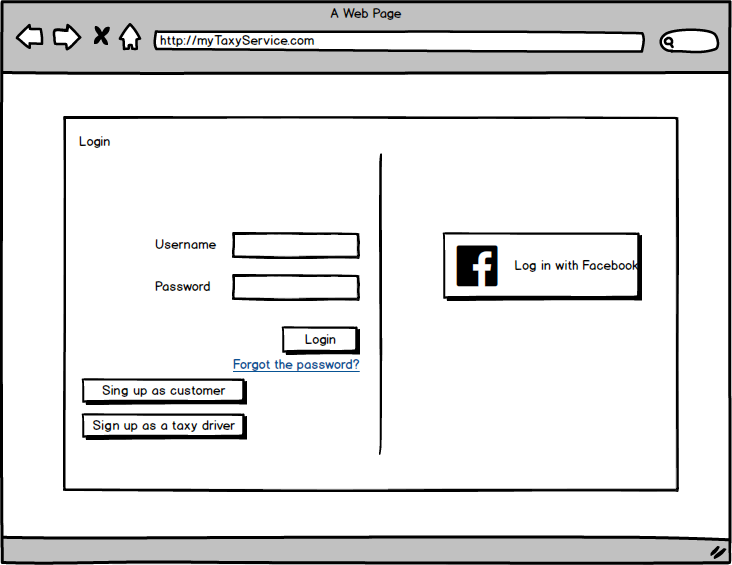
\includegraphics[scale=0.4]{IMG/UserInterfaces/CustomerLogin.png}
			
			
			\end{center}
			\begin{center}
			
			
			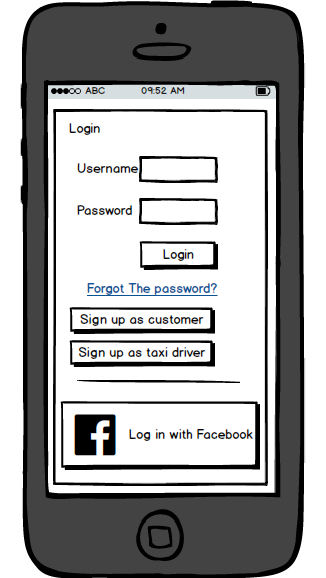
\includegraphics[scale=0.4]{IMG/UserInterfaces/CustomerLogin_m.png}
			\end{center}

		\subsection{Hardware Interfaces}
		Since mobile and web applications don't have any dedicated hardware we have not designed any hardware interfaces for our system.
		The interaction with the central database is performed by connections handled by the already installed operating system on the mobile devices or the users computers.

		\subsection{Software Interfaces}
			\begin{itemize}
				\item The mobile application communicates with the GPS application in order to get geographical informations about the user.
				
				\item The web application communicates with the browser in order to get geographical informations about the user.
				
				\item Mobile and web applications communicates with the database through HTTP requests to the server.
			\end{itemize}

		\subsection{Interfaces to Others Application}
			\begin{itemize}
				\item myTaxiService web application require that at least one of these browsers is installed on the user Personal Computer:
			
					\begin{center}
						\begin{table}[h!]
							
							\begin{center}
								\caption{Browsers}
								\label{tab:browsersTable}

								\begin{tabular}{cccc}
									\toprule
									\textbf{Name} & \textbf{Version} & \textbf{Company} & \textbf{Source}\\
									\midrule
									Safari & 9.0.1 & Apple Inc. & \href{http://www.apple.com/safari/}{Get Safari}\\
									\midrule
									Firefox & 41.0 & Mozilla & \href{https://www.mozilla.org/en-US/firefox/new/}{Get Firefox}\\
									\midrule
									Chrome & 46.0.2490 & Google & \href{https://www.google.com/chrome/browser/desktop/}{Get Chrome}\\
									\midrule
									Microsofr Edge & 20.10240.16384.0 & Microsoft & \href{https://www.microsoft.com/en-us/download/details.aspx?id=48126}{Get Edge}\\
									\bottomrule
								\end{tabular}
							\end{center}
							
						\end{table}
					\end{center}

				\item myTaxiService mobile application require that at least one of these operating systems is installed on the user Smartphone:

					\begin{center}
						\begin{table}[h!]
							
							\begin{center}
								\caption{Mobile Operative Systems}
								\label{tab:mobileOSTable}

								\begin{tabular}{cccc}
									\toprule
									\textbf{Name} & \textbf{Version} & \textbf{Company} & \textbf{Source}\\
									\midrule
									Android & KitKat 4.4W.2 or later & Google & \href{https://www.android.com}{Android Info}\\
									\midrule
									iOS & 9.1 or later & Apple Inc. & \href{http://www.apple.com/ios/}{iOS Info}\\
									\midrule
									Windows 10 & 10.0.10572.0 or later & Microsoft & \href{http://www.microsoft.com/it-it/mobile/windows10/?dcmpid=omc-org-globalsite.globalredirect}{Windows 10 Info}\\
									\bottomrule
								\end{tabular}
							\end{center}
							
						\end{table}
					\end{center}

				\item To give an additional LogIn method, we use also the "LogIn with Facebook" API relased by Facebook. Facebook Login for Apps is a fast and convenient way for people to create accounts and log into our system across multiple platforms. It is well described at \href{https://developers.facebook.com/docs/facebook-login}{Facebook Login API Page.}
			\end{itemize}


		\subsection{Communication Interfaces}
		The communication between system pieces is not specified because it is handled by the underlying operating systems for both the mobile application and the web portal.

		In particular, the web and mobile applictaions will communicate with the server through HTTP/HTTPS requests. 

			\begin{itemize}
				\item HTTP communicate through the port number 80 and is handled by the operating system. 
				\item HTTPS communicate through the port number 443 and is handled by the operating system.
			\end{itemize}

	\section{Functional Requirements}
	In this section are described, for every Actor, the Functional Requirements needed to reach the linked Goal.

		\subsection{Functional Requirements for Guest Users}
		Here are listed all the Functional Requirements referring to the Goals that affects Guest Users.

			\subsubsection{\lbrack \hyperref[sec:g1_1_1]{G1.1.1 - Allow guest users to become a customer creating a myTaxiService Account}\rbrack}
			To allow the guest user to perform a successful registration the system has to:

				\begin{itemize}
					\item \lbrack Req.1\rbrack \label{sec:fr1_g1_1_1} check if the selected username has not already been taken by another user to perform a successful registration.
					\item \lbrack Req.2\rbrack \label{sec:fr2_g1_1_1} check if the selected password is at least 8 characters long.
					\item \lbrack Req.3\rbrack \label{sec:fr3_g1_1_1} check if the selected password contains either digits and alphabetic characters.
					\item \lbrack Req.4\rbrack \label{sec:fr4_g1_1_1} The Guest User must use an email that has not already been used by another one.
					\item \lbrack Req.5\rbrack \label{sec:fr5_g1_1_1} Guest Users can only access to the registration forms and login page.
					\item \lbrack Dom.1\rbrack \label{sec:da1_g1_1_1} The email used by the Guest User is a valid one.
				\end{itemize}

			\subsubsection{\lbrack \hyperref[sec:g1_1_2]{G1.1.2 - Allow guests user to become a customer using his Facebook Account}\rbrack}
			To reach this goal, we think that these requirements are needed:

				\begin{itemize}
					\item \lbrack Req.1\rbrack \label{sec:fr1_g1_1_2} The Guest User must be connected to the Internet in some way.
					\item \lbrack Req.2\rbrack \label{sec:fr2_g1_1_2} The Guest User cannot be already registered as a Customer.
					\item \lbrack Req.3\rbrack \label{sec:fr3_g1_1_2} The Guest User must select an username that has not already been selected by another one.
					\item \lbrack Req.4\rbrack \label{sec:fr4_g1_1_2} The Guest User must have a valid Facebook Account.
					\item \lbrack Req.5\rbrack \label{sec:fr5_g1_1_2} Guest Users can only access to the registration forms and login page.
					
					* Note that the email is validated by Facebook when the User create his Facebook Account.
				\end{itemize}

			\subsubsection{\lbrack \hyperref[sec:g1_2]{G1.2 Allow guest users to become a taxi driver}\rbrack}
			To reach this goal, we think that these requirements are needed:

				\begin{itemize}
					\item \lbrack Req.1\rbrack \label{sec:fr1_g1_2} The Guest User must be connected to the Internet in some way.
					\item \lbrack Req.2\rbrack \label{sec:fr2_g1_2} The Guest User cannot be already registered as a Taxi Driver.
					\item \lbrack Req.3\rbrack \label{sec:fr3_g1_2} The Guest User must select an username that has not already been selected by another one.
					\item \lbrack Req.4\rbrack \label{sec:fr4_g1_2} Guest Users can only access to the registration forms and login page.
					\item \lbrack Req.5\rbrack \label{sec:fr5_g1_2} The Guest User must use an email that has not already been used by another one.
					\item \lbrack Req.6\rbrack \label{sec:fr6_g1_2} Guest Users has to provide a Taxi Licence that has not already been used by another one.
					\item \lbrack Dom.1\rbrack \label{sec:da1_g1_2} The email used by the Guest User is a valid one.
				\end{itemize}

		\subsection{Functional Requirements for Registered Users}

			\subsubsection{\lbrack \hyperref[sec:g2_1]{G.2.1 Allow registered users to log in with myTaxiService account.}\rbrack}
			To reach this goal, we think that these requirements are needed:

				\begin{itemize}
					\item \lbrack Req.1\rbrack \label{sec:fr1_g2_1} The Registered User must be registered with a myTaxiService account.
					\item \lbrack Req.2\rbrack \label{sec:fr2_g2_1} The Registered User must be in posses of his username and password to successful login.
					\item \lbrack Req.3\rbrack \label{sec:fr3_g2_1} The Registered User must insert valid username and password to successful login.
					\item \lbrack Req.4\rbrack \label{sec:fr4_g2_1} The Registered User cannot access to the other functions of the system before a successful login.
				\end{itemize}

		\subsection{Functional Requirements for Customers}

			\subsubsection{\lbrack \hyperref[sec:g2_2]{G.2.2 Allow customers to log in with Facebook account.}\rbrack}
			To reach this goal, we think that these requirements are needed:

				\begin{itemize}
					\item \lbrack Req.1\rbrack \label{sec:fr1_g2_2} The Customer must be registered with a Facebook account.
					\item \lbrack Req.2\rbrack \label{sec:fr2_g2_2} The Customer cannot access to the other functions of the system before a successful Facebook Login.
					\\

					* Note that all te requirements concerning the validity of username and password are already checked by the Facebook Login System. 
				\end{itemize}

			\subsubsection{\lbrack \hyperref[sec:g3]{G.3 Allow customers to require a taxi.}\rbrack}
			To reach this goal, we think that these requirements are needed:

				\begin{itemize}
					\item \lbrack Req.1\rbrack \label{sec:fr1_g3} The Customer must be already registered and logged in with a myTaxiService account or a Facebook Account.
					\item \lbrack Req.2\rbrack \label{sec:fr2_g3} The Customer must be on the require-a-taxi page.
					\item \lbrack Req.3\rbrack \label{sec:fr3_g3} The Customer must push the button to require a taxi.
					\item \lbrack Dom.1\rbrack \label{sec:da1_g3} Location of the request is the Customer current location.
				\end{itemize}

			\subsubsection{\lbrack \hyperref[sec:g4]{G.4 Allow customers to reserve a ride.}\rbrack}
			To reach this goal, we think that these requirements are needed:

				\begin{itemize}
					\item \lbrack Req.1\rbrack \label{sec:fr1_g4} The Customer must be already registered and logged in with a myTaxiService account or a Facebook Account.
					\item \lbrack Req.2\rbrack \label{sec:fr2_g4} The Customer must be on the reserve-a-ride page.
					\item \lbrack Req.3\rbrack \label{sec:fr3_g4} The Customer must provide a valid starting location different from the ending location.
					\item \lbrack Req.4\rbrack \label{sec:fr4_g4} The Customer must provide a valid ending location different from the starting location.
					\item \lbrack Req.5\rbrack \label{sec:fr5_g4} The Customer must provide a reservation time that is at least two hour after the current time.
				\end{itemize}

			\subsubsection{\lbrack \hyperref[sec:g5]{G.5 Allow customers to delete a previous reservations.}\rbrack}
			To reach this goal, we think that these requirements are needed:

				\begin{itemize}
					\item \lbrack Req.1\rbrack \label{sec:fr1_g5} The Customer must be already registered and logged in with a myTaxiService account or a Facebook Account.
					\item \lbrack Req.2\rbrack \label{sec:fr2_g5} The Customer must be on the reserved-rides page.
					\item \lbrack Req.3\rbrack \label{sec:fr3_g5} The Customer must push the delete button relative to the desired reservation.
					\item \lbrack Dom.1\rbrack \label{sec:da1_g5} The reservation is deleted after the Customer action.
				\end{itemize}

		\subsection{Functional Requirements for Taxi Drivers}

			\subsubsection{\lbrack \hyperref[sec:g6]{G.6 Allow taxi drivers to accept or decline a ride request.}\rbrack}
			To reach this goal, we think that these requirements are needed:

				\begin{itemize}
					\item \lbrack Req.1\rbrack \label{sec:fr1_g6} The Taxi Driver must be already registered and logged in with a myTaxiService account.
					\item \lbrack Req.2\rbrack \label{sec:fr2_g6} The Taxi Driver 
				\end{itemize}


	\section{Scenarios}


	\section{UML Models}

		\subsection{Use-Case Diagrams}

		\subsection{Class Diagrams}

		\subsection{State Machine Diagrams}

	\section{Non Functional Requirements}

		\subsection{Performance Requirements}

		\subsection{Design Constraints}

		\subsection{Software System Attributes}

			\subsubsection{Avaiability}

			\subsubsection{Maintainability}

			\subsubsection{Portability}

		\subsection{Security}

			\subsubsection{External Interface Side}

			\subsubsection{Application Side}

			\subsubsection{Server Side}


\chapter{Appendix}
//TODO
\end{document}